%&pdflatex
\documentclass{standalone}
%\documentclass[a4paper, landscape]{article}
\usepackage{graphicx}
\usepackage{pbox}

\newcommand{\picHeight}{1in}
\begin{document}

        \begin{tabular}{| c | c | c | c | c |}
            \hline
            \pbox{20cm}{Config-\\uration} &
            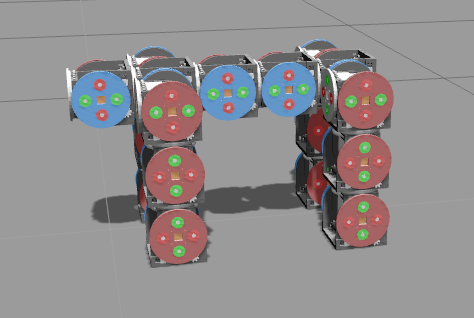
\includegraphics[height=\picHeight]{walk4.png} &
            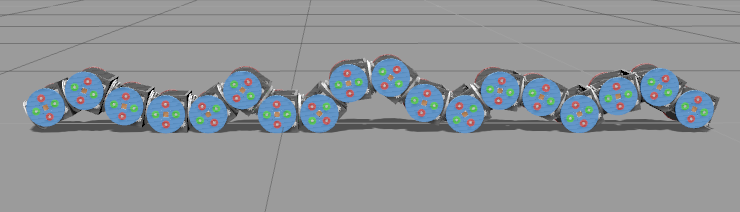
\includegraphics[height=\picHeight]{snake18.png} &
            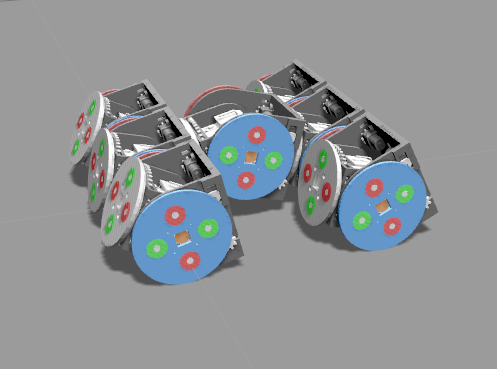
\includegraphics[height=\picHeight]{car.png} &
            
\includegraphics[height=\picHeight]{robot-character.jpg} 
             \\ 
            ~ & WALK4 & SNAKE18 & CAR & DRIVER5 \\ \hline
            Components &
            \pbox{20cm}{BODY3 \\ LEG3 \(\times4\)} &
            \pbox{20cm}{SNAKE3 \(\times6\)} &
            \pbox{20cm}{STEER3 \\ DRIVER1 \(\times4\)} &
            \pbox{20cm}{STEER3 \\ DRIVER1 \(\times2\)}
            \\ \hline
            Behaviors &
            \pbox{20cm}{\(Walk(t)\)} &
            \pbox{20cm}{\(Slither()\)} &
            \pbox{20cm}{\(DRIVE(v,t)\) \\ \(TURN(\theta)\)} &
            \pbox{20cm}{\(DRIVE(v,t)\) \\ \(TURN(\theta)\)}
            \\ \hline
        \end{tabular}
\end{document}








